Dalam praktek membuat whatsapp chatbot ini, hal pertama yang harus dilakukan adalah mengenal bahasa pemrograman Python dan mengetahui tentang software yang digunakan yaitu Anaconda3.

\section{Sejarah Python}
Nama python berasal dari acara televisi Monty python's flying circus. Python merupakan bahasa pemrograman yang dikembangkan oleh Guido Van Rossum pada tahun 1990 di CWI, Amsterdam. bahasa ini merupakan lanjutan dari bahasa pemrograman ABC. pada tahun 1995, Guido pindah ke CNRI dan mengeluarkan python versi 1.6. pada tahun 2000, Guido pindah ke BeOpen dan mengeluarkan python versi 2.0 setelah itu Guido dan tim PythonLabs pindah ke  DigitalCreations. saat ini Guido dan Python Software Foundation terus melakukan perkembangan hingga python versi 2.6.1 dan python versi 3.0
Python Software Foundation merupakan sebuah organisasi yang memiliki hak atas bahasa pemrograman python, hal ini dilakukan untuk mencegah bahasa pemrograman python dimiliki oleh perusahaan komersial.

\subsection{Perbedaan Python 2 dan 3}
Perbedaan Python 2 dan Python 3 dapat dilihat pada gambar berikut.
\begin{figure}[!htbp]
        \centerline{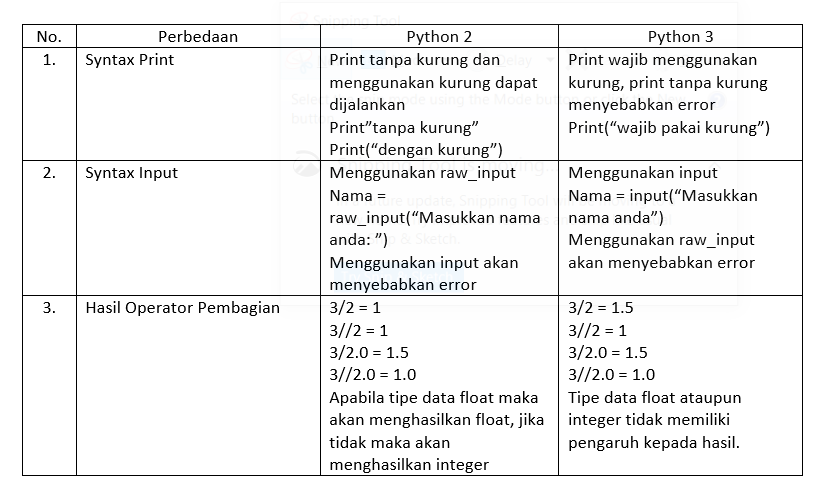
\includegraphics[scale=.75]{figures/perbedaan}}
        \caption{Perbedaan Python 2 dan Python 3}
		\label{perbedaan}
\end{figure}

\subsection{Tipe Data}
\begin{enumerate}
 \item Numbers\\
 Tipe numerik pada Python dibagi menjadi 3: int, float, complex
 \begin{verbatim}
a = 5
print(a, "is of type", type(a))
a = 2.0
print(a, "is of type", type(a))
a = 1+2j
print(a, "is complex number?", isinstance(1+2j,complex))
 \end{verbatim}
 
 Output:
 \begin{verbatim}
 5 is of type <class 'int'>
2.0 is of type <class 'float'>
(1+2j) is complex number? True
 \end{verbatim}
 Integer tidak dibatasi oleh angka atau panjang tertentu, namun dibatasi oleh memori yang tersedia. Sehingga Anda tidak perlu menggunakan variabel yang menampung big number misalnya long long (C/C++), biginteger, atau sejenisnya. Contoh kode untuk menunjukkan bahwa Python tidak membatasi output integer adalah pencarian bilangan ke-10.000 pada deret fibonacci (catatan: bilangan ke-10.000 pada deret fibonacci memiliki panjang 2.090 digit) sebagai berikut:
 \begin{verbatim}
 x=[0]*10005;              #inisialisasi array 0 sebanyak 10005; x[0]=0
x[1]=1;                   #x[1]=1
 
for j in range(2,10001):
      x[j]=x[j-1]+x[j-2]  # Fibonacci
print(x[10000])
 \end{verbatim}
 Output:\\
 33644764876431783266621612005107543310302148460680063906564769974680081442166662368155595513633734025\\
 Perhatikan bagaimana Python melakukan pemotongan pada digit ke 16 pada variabel float b.Float atau bilangan pecahan dibatasi akurasinya pada 15 desimal. Yang membedakan Integer dan Float adalah titik (decimal points). Misalnya dalam penulisan angka 1 jenisnya Integer, tapi jika dituliskan sebagai 1.0 artinya berjenis Float atau pecahan.
 \begin{verbatim}
 b = 0.1234567890123456789
b
 \end{verbatim}
 Output:\\
 0.12345678901234568
 
 Karena Python banyak digunakan juga oleh matematikawan, tipe bilangan di Python juga mendukung bilangan imajiner dan bilangan kompleks. Nilai bilangan kompleks (complex) dituliskan dalam formulasi x + yj, yakni bagian x adalah bilangan real, dan y adalah bilangan imajiner. Contohnya adalah sebagai berikut:
 \begin{verbatim}
 a = 1234567890123456789
a
 \end{verbatim}
 Output:\\
 1234567890123456789
 
 \begin{verbatim}
 c = 1+2j
c
 \end{verbatim}
 Output:\\
 (1+2j)
 \item Strings\\
 String adalah urutan dari karakter unicode. Dideklarasikan dengan petik tunggal atau ganda. String >1baris dapat ditandai dengan tiga petik tunggal atau ganda ''' atau """.
 \begin{verbatim}
 s = "This is a string"
s = '''this is a multiline
next new line (1)
another new line (2)'''
 \end{verbatim}
 Seperti list dan tuple, slicing operator [ ] dapat digunakan pada string. Sebuah string utuh bersifat mutable, namun elemennya bersifat immutable.
 \begin{verbatim}
 s = "Hello World!"
print(s[4])
print(s[6:11])
s[5]="d"
 \end{verbatim}
 Output:
 \begin{verbatim}
 'o'
'World'
Traceback (most recent call last):
  File "<stdin>", line 1, in <module>
TypeError: 'str' object does not support item assignment
 \end{verbatim}
 \begin{verbatim}
 s = "Hello World!"
print(s)
s= "Try Python!"
print(s)
 \end{verbatim}
 Output:
 \begin{verbatim}
 'Hello World!'
'Try Python!'
 \end{verbatim}
 
 \item Bool/Boolean\\
 Tipe data bool atau Boolean, merupakan turunan dari bilangan bulat (integer atau int) yang hanya punya dua nilai konstanta: True dan False.\\

Nilai Boolean\\
Nilai konstanta False dan True merepresentasikan nilai kebenaran (truth values), meskipun ada nilai-nilai lain yang juga dianggap benar atau salah. Di dalam konteks angka, misalnya digunakan sebagai argumen dari operator matematika aritmatika, kedua nilai ini berlaku seperti halnya bilangan bulat 0 dan 1, sesuai False dan True.\\

Ada fungsi bawaan bool() yang dapat mengubah nilai menjadi nilai Boolean, apabila nilai tersebut dapat direpresentasikan sebagai nilai kebenaran (truth values). \\

Nilai kebenaran adalah sebuah nilai yang dapat diuji sebagai benar atau salah, untuk digunakan di sintaksis kondisi if atau while atau sebagai operan dari operasi Boolean.\\

Berikut adalah objek bawaan yang didefinisikan bernilai salah dalam pengujian nilai kebenaran:
\begin{enumerate}
\item Konstanta yang sudah didefinisikan bernilai salah: None dan False
\item Angka nol dari semua tipe numeric: 0, 0.0, 0j, Decimal(0), Fraction(0, 1)
\item Urutan (sequence) dan koleksi (collection) yang kosong: '', (), {}, set(), range(0)
\end{enumerate}
Untuk objek yang didefinisikan sendiri, representasi nilai Boolean akan bergantung dari definisi metode (method) khusus bernama \_\_bool\_\_(self). Jika metode ini mengembalikan True maka interpretasi nilai dari objeknya akan True, demikian juga sebaliknya.
Operasi Boolean\\
Operasi dan fungsi bawaan yang memiliki hasil Boolean akan selalu mengembalikan 0 atau False untuk yang bernilai salah, serta 1 atau True untuk yang bernilai benar, kecuali dinyatakan berbeda dalam dokumentasi.\\

Operasi untuk tipe Boolean akan dijelaskan lebih lanjut di modul Operator, Operands, dan Expressions.

\item List\\
List adalah jenis kumpulan data terurut (ordered sequence), dan merupakan salah satu variabel yang sering digunakan pada Python. Serupa, namun tak sama dengan array pada bahasa pemrograman lainnya. Bedanya, elemen List pada Python tidak harus memiliki tipe data yang sama. Mendeklarasikan List cukup mudah dengan kurung siku dan elemen yang dipisahkan dengan koma. Setiap data didalamnya dapat diakses dengan indeks yang dimulai dari 0.
\begin{verbatim}
a = [1, 2.2, 'python']
\end{verbatim}
Python mengenal slicing operator [] yang dapat melakukan ekstraksi sebuah item atau beberapa item yang berada dalam range tertentu pada tipe data urutan (sequences), misalnya list, string dan tuple. Beberapa tipe urutan juga mendukung "extended slicing" dengan parameter ketiga berupa "step".\\
x[0] artinya mengambil elemen paling awal, dengan index 0 dari List x\\

x[5] artinya mengambil elemen dengan index 5 dari List x\\

x[-1] artinya mengambil elemen dengan index paling belakang ke-1 dari List x\\

x[3:5] artinya membuat list dari anggota elemen List x dengan index 3 hingga sebelum index 5 (tidak termasuk elemen dengan index 5, dalam hal ini hanya index 3-4)\\

x[:5] artinya membuat list dari anggota elemen List x paling awal hingga sebelum index 5 (tidak termasuk elemen dengan index 5, dalam hal ini hanya index 0-4)\\

x[-3:] artinya membuat list dari anggota elemen List x mulai index ke-3 dari belakang hingga paling belakang\\

x[1:7:2] artinya membuat list dari anggota elemen List x dengan index 1 hingga sebelum index 5, dengan "step" 2 (dalam hal ini hanya index 1, 3, 5)
\begin{verbatim}
x = [5,10,15,20,25,30,35,40]
print(x[5])
print(x[-1])
print(x[3:5])
print(x[:5])
print(x[-3:])
print(x[1:7:2])
\end{verbatim}
Output:
\begin{verbatim}
30
40
[20, 25]
[5, 10, 15, 20, 25]
[30, 35, 40]
[10, 20, 30]
\end{verbatim}

Elemen pada list dapat diubah atau ditambahkan. Misalnya untuk melakukan perubahan kemudian penambahan:
\begin{verbatim}
x = [1,2,3]
x[2]=4
x
\end{verbatim}
Output:
\begin{verbatim}
[1, 2, 4]
\end{verbatim}
\begin{verbatim}
x.append(5)
x
\end{verbatim}
Output:
\begin{verbatim}
[1, 2, 4, 5]
\end{verbatim}

Untuk menghapus, gunakan fungsi del
\begin{verbatim}
spam = ['cat', 'bat', 'rat', 'elephant']
del spam[2]
spam
\end{verbatim}
Output:
\begin{verbatim}
['cat', 'bat', 'elephant']
\end{verbatim}

\begin{verbatim}
del spam[2]
spam
\end{verbatim}
Output:
\begin{verbatim}
['cat', 'bat']
\end{verbatim}

\item Tuple\\
Tuple adalah jenis dari list yang tidak dapat diubah elemennya. Umumnya tuple digunakan untuk data yang bersifat sekali tulis, dan dapat dieksekusi lebih cepat. Tuple didefinisikan dengan kurung dan elemen yang dipisahkan dengan koma.
\begin{verbatim}
t = (5,'program', 1+3j)
\end{verbatim}
Seperti list, kita dapat melakukan slicing, namun pada tuple kita tidak dapat melakukan perubahan:
\begin{verbatim}
t = (5,'program', 1+3j)
t[1]
t[0:3]
t[0]=10
\end{verbatim}
Output:
\begin{verbatim}
'program'
(5, 'program', (1+3j))
Traceback (most recent call last):
  File "<stdin>", line 1, in <module>
TypeError: 'tuple' object does not support item assignment
\end{verbatim}


\item Set\\
Set adalah kumpulan item bersifat unik dan tanpa urutan (unordered collection). Didefinisikan dengan kurawal dan elemennya dipisahkan dengan koma. Pada Set kita dapat melakukan union dan intersection, sekaligus otomatis melakukan penghapusan data duplikat.

\begin{verbatim}
a = {1,2,2,3,3,3}
a
\end{verbatim}
Output:
\begin{verbatim}
{1, 2, 3}
\end{verbatim}

Karena set bersifat unordered, maka kita tidak bisa mengambil sebagian data / elemen datanya menggunakan proses slicing.
\begin{verbatim}
a = {1,2,3}
a[1]
\end{verbatim}
Output:
\begin{verbatim}
Traceback (most recent call last):
 File "<string>", line 301, in runcode
 File "<interactive input>", line 1, in <module>
TypeError: 'set' object does not support indexing
\end{verbatim}

\item Dictionary\\
Dictionary pada Python adalah kumpulan pasangan kunci-nilai (pair of key-value) yang bersifat tidak berurutan. Dictionary dapat digunakan untuk menyimpan data kecil hingga besar. Untuk mengakses datanya, kita harus mengetahui kuncinya (key). Pada Python, dictionary didefinisikan dengan kurawal dan tambahan definisi berikut:
\begin{enumerate}
\item Setiap elemen pair key-value dipisahkan dengan koma (,)
\item Key dan Value dipisahkan dengan titik dua (:)
\item Key dan Value dapat berupa tipe variabel/obyek apapun
\end{enumerate}

\begin{verbatim}
d = {1:'value','key':2}
print(type(d))
\end{verbatim}
Output:
\begin{verbatim}

<class 'dict'>

\end{verbatim}

\begin{verbatim}
d = {1:'value','key':2}
print(type(d))
print("d[1] = ", d[1]);
print("d['key'] = ", d['key']);
\end{verbatim}

Output:
\begin{verbatim}
<class 'dict'>
d[1] = value
d['key'] =  2
\end{verbatim}
Dictionary bukan termasuk dalam implementasi urutan (sequences), sehingga tidak bisa dipanggil dengan urutan indeks. Misalnya dalam contoh berikut dicoba dengan indeks 2, tetapi menghasilkan error (KeyError) karena tidak ada kunci (key) 2:

\begin{verbatim}
d = {1:'value','key':2}
print(type(d))
print("d[1] = ", d[1]);
print("d['key'] = ", d['key']);
 
# Generates error
print("d[2] = ", d[2]);
\end{verbatim}

Output:
\begin{verbatim}
<class 'dict'>
d[1] = value
d['key'] = 2

---------------------------------------------------------------------------
KeyError Traceback (most recent call last)
<ipython-input-7-4b566e677ca2> in <module>()
1 d = {1:'value','key':2}
----> 2 print("d[2] = ", d[2]);

KeyError: 2
\end{verbatim}

\end{enumerate}

\subsection{Konversi antar tipe data}
Kita dapat melakukan konversi tipe data bawaan dengan menggunakan fungsi konversi tipe bawaan (standard type) misalnya: int(), float(), str(), dll.
Contoh:\\
float(5)\\
Output:\\
5.0\\
Konversi float ke int akan bersifat floor/truncating, menghilangkan nilai di belakang koma.\\
Contoh:\\
int(10.6)\\
Output:\\
10\\
int(-10.6)\\
Output:\\
-10\\
Konversi dari-dan-ke string akan melalui pengujian dan dipastikan validitasnya.\\
float('2.5')\\
Output:\\
2.5\\
str(25)\\
Output:\\
'25'\\
int('1p')\\
Output:
\begin{verbatim}
Traceback (most recent call last):
 File "<string>", line 301, in runcode
 File "<interactive input>", line 1, in <module>
ValueError: invalid literal for int() with base 10: '1p'
\end{verbatim}

Anda juga dapat melakukan konversi kumpulan data (set, list, tuple).\\
set([1,2,3])\\
Output:\\

{1, 2, 3}\\
tuple({5,6,7})\\
Output:\\

(5, 6, 7)\\
list('hello')\\
Output:\\

['h', 'e', 'l', 'l', 'o']\\

Untuk konversi ke dictionary, data harus memenuhi persyaratan key-value. Berikut adalah dua contoh konversi:\\
List dari beberapa List yang isinya pasangan nilai menjadi Dictionary. \\

Serta konversi List dari beberapa Tuple yang isinya pasangan nilai menjadi Dictionary.\\
dict([[1,2],[3,4]])\\
Output:\\

{1: 2, 3: 4}\\
dict([(3,26),(4,44)])\\
Output:\\

{3: 26, 4: 44}\\









\subsection{Implementasi dan Penggunaan Python di Perusahaan Dunia}
\begin{enumerate}
\item spotify 
\par
spotify adalah suatu layanan musik streaming yang menggunakan pemrograman python untuk analisis data dan backend. pada backend spotify berkomunikasi dengan 0MQ. 0MQ itu sendiri  adalah suatu framework dan library open source untuk networking. untuk analisis data tersebut spotify menggunakan luigi, dan modul python yang sinkron dengan hadoop.
\item Google
\par 
Google ini sudah menggunakan bahasa pemprograman python ini sudah sajak dari awal berdirinya. Dan pada saat ini bahasa pemprograman python merupakan salah satu bahasa pemprograman server-side resmi di google. Meskipun ada script yang ditulis untuk google menggunakan bahasa perl dan bash, maka nantinya script tersebut akan diubah ke python terlebih dahulu, karena kemudahan dalam perawatannya.
\item Industrial Light and Magic
\par 
Industrial Light and Magic ini merupakan studio special efek yang dibutuhkan untuk film star wars saja. Karena infrastruktur awal industrial light and magisc ini menggunakan C dan C++, maka akan lebih mudah mengintegrasikan bahasa pemprograman python ketimbang bahasa pemprograman lainnya. Dengan menggunakan bahasa pemprogramana python ini industrial light and magic dengan mudah membungkus komponen software dan dapat meningkatkan aplikasi grafisnya.
\item Netflix
\par 
Netflix adalah suatu layanan pemutaran film yang dapat dilakukan oleh pengguna dimanapun dan kapanpun. Pada netfilx bahasa pemprograman yang digunakan adalah bahasa pemprograman python, bahasa pemprograman ini digunakan pada Central Alert Gateway yang akan me-reroute alert dan mengirimkannya pada individu yang akan melihatnya serta juga  dapat secara otomatis reboot atau menghentikan proses yang dianggap bermasalah. Selain itu python juga digunakan untuk menelusuri riwayat dan perubahan pengaturan keamanan.
\item instagram 
\par 
Instagram adalah suatu aplikasi mobile berbasis IOS, android dan windows phone, dimana pengguna dapat berbagi foto dan video melalui instagram ini. Pada instagram ini menggunakan bahasa pemprograman python dalam task queuennya atau fitur dimana setiap pengguna dapat berbagi foto atau video ke beberapa social network lainnya seperti facebook, twitter, dan lain-lainnya.

\end{enumerate}

\subsection{Jenis-Jenis Variabel}
Variabel merupakan tempat penyimpanan data. Tipe data merupakan jenis data yang tersimpan di dalam variabel. terdapat aturan dalam penulisan Variabel.
\begin{enumerate}
 \item Nama variabel diawali dengan huruf atau garis bawah, contoh: nama, \_nama, namaKu, nama\_variabel.
 \item Karakter selanjutnya dapat berupa huruf, garis bawah atau angka, contoh: \_\_nama, nama1, p1.
 \item Karakter bersifat case-sensitive (huruf besar dan huruf kecil dibedakan), contoh: Nama dan NAMA keduanya adalah variabel yang berbeda.
 \item Nama variabel tidak boleh menggunakan kata kunci yang ada pada bahasa pemrograman python, contoh: if, else, while
 \item Nama variabel tidak boleh diawali dengan angka
\end{enumerate}

Jenis-jenis tipe data pada python.
Tipe Data Primitif, dibagi menjadi 3 yaitu:
\begin{enumerate}
 \item Tipe data integer (angka), penulisannya tidak membutuhkan tanda petik, contoh: 10 atau 15
 \item Tipe data string (teks), tipe data string ditandai dengan teks yang diapit oleh tanda petik (""), contoh: "nama saya adalah dinda majesty"
 \item Tipe data boolean (memiliki dua nilai yaitu true dan false atau 0 dan 1)
\end{enumerate}

Contoh penulisan variabel dan tipe datanya:
\begin{enumerate}
 \item angka = 10, angka merupakan nama variabel sedangkan 10 adalah nilai dari variabel yang tipe datanya integer.
 \item nama = "Dinda Majesty", nama merupakan nama variabel sedangkan "Dinda Majesty" merupakan nilai dari variabel yang tipe datanya string, ditandai dengan adanya petik ("").
 \item makan = True , makan merupakan nama variabel sedangkan True merupakan nilai dari variabel yang tipe datanya boolean.
\end{enumerate}

\subsection{Input dan Output}
Berikut kode untuk meminta inputan dari user.
\lstinputlisting[caption=Input dan Output , language=Python, firstline=7, lastline=10]{src/teori.py}
Perintah input() berguna untuk meminta inputan dari user, sehingga memungkinkan user untuk menginputkan data.\\
Perintah print() berguna untuk menampilkan output dari data yang diinputkan oleh user, sehingga data yang diinputkan user dapat ditampilkan ke layar.

\subsection{Operator Aritmatika dan Konversi Tipe Data}
Operator aritmatika
\begin{enumerate}
 \item penjumlahan (+)
 \item pengurangan (-)
 \item perkalian (*)
 \item pembagian (/)
 \item sisa bagi/modulus (%)
 \item pemangkatan (**)
\end{enumerate}
Cara melakukan perubahan terhadap tipe data string menjadi integer, contoh: variabel = "10". Kita dapat mengubah string "10" menjadi angka 10 dengan menambahkan kode int(variabel), dengan begitu 10 yang awalnya bertipe data string akan dikonversikan menjadi integer.\\
Cara melakukan perubahan terhadap tipe data integer menjadi string, contoh: variabel = 150. Kita dapat mengubah integer 150 menjadi string "150" dengan menambahkan kode str(variabel), maka tipe data dari variabel akan dikonversikan menjadi string.

\subsection{Perulangan}
perulangan terdiri atas 3 kondisi.
\begin{enumerate}
 \item While, apabila kondisinya True, maka perulangan akan terus berjalan hingga diperoleh kondisi False. Contoh penggunaan while:\\
\lstinputlisting[caption=While Loop , language=Python, firstline=12, lastline=18]{src/teori.py}
 \item For, perulangan for bisa melakukan perulangan terhadap item apapun seperti list atau string. Contoh penggunaan For:\\
\lstinputlisting[caption=For Loop , language=Python, firstline=20, lastline=23]{src/teori.py}
 \item nested, perulangan ini memungkinkan adanya perulangan didalam perulangan. Contoh penggunaan nested:\\
\lstinputlisting[caption=Nested Loop , language=Python, firstline=25, lastline=35]{src/teori.py}
\end{enumerate}
Pada penulisan sintaks While dan For harus memperhatikan identasi (baris yang menjorok ke dalam), jika tidak diperhatikan dengan baik maka akan terjadi error terhadap identasi. Untuk menambahkan identasi dapat menggunakan spasi atau tab.

\subsection{Looping For}
Seperti di bahasa pemrograman lainnya, Python juga memiliki fungsi for. Bedanya di Python, For tidak hanya untuk perulangan dengan jumlah finite (terbatas), melainkan lebih ke fungsi yang dapat melakukan perulangan pada setiap jenis variabel berupa kumpulan atau urutan. Variabel yang dimaksud bisa berupa list, string, ataupun range. Jika sebuah list atau urutan berisi expression, maka Ia akan dievaluasi terlebih dahulu. Kemudian item pertama pada urutan atau list akan diassign sebagai variabel iterating\_var. Setelahnya, blok statement akan dieksekusi, berlanjut ke item berikutnya, berulang, hingga seluruh urutan habis.
contoh for:
\begin{verbatim}
for letter in 'Python':  # First Example
    print('Current Letter: {}'.format(letter))
fruits = ['banana', 'apple', 'mango']
for fruit in fruits:  # Second Example
    print('Current fruit: {}'.format(fruit))
\end{verbatim}
Output:
\begin{verbatim}
Current Letter : P
Current Letter : y
Current Letter : t
Current Letter : h
Current Letter : o
Current Letter : n
Current fruit : banana
Current fruit : apple
Current fruit : mango
\end{verbatim}
Anda juga dapat melakukan perulangan berdasarkan indeks atau range dengan memanfaatkan fungsi len():
\begin{verbatim}
fruits = ['banana', 'apple', 'mango']
for index in range(len(fruits)):
    print('Current fruit: {}'.format(fruits[index]))
\end{verbatim}
Output:
\begin{verbatim}
Current fruit : banana
Current fruit : apple
Current fruit : mango
\end{verbatim}

\subsection{While}
While pada bahasa Python digunakan untuk mengeksekusi statement selama kondisi yang diberikan terpenuhi (True). Kondisi dapat berupa expression apapun, dan harap diingat bahwa True di Python termasuk semua nilai non-zero. Saat kondisi menjadi False, program akan melanjutkan ke baris setelah blok statement.\\
Seperti for dan semua statement percabangan, blok statement yang mengikuti kondisi while dan memiliki posisi indentasi yang sama, dianggap blok statement yang akan dieksekusi.

Contoh:
\begin{verbatim}
count = 0
while (count < 5):
    print('The count is: {}'.format(count))
    count = count + 1
\end{verbatim}
Output:
\begin{verbatim}
The count is: 0
The count is: 1
The count is: 2
The count is: 3
The count is: 4
\end{verbatim}
Seperti pada bahasa lainnya, eksekusi statement while mungkin bersifat infinit / infinite loop saat sebuah kondisi tidak pernah bernilai False. Contohnya sebagai berikut:
\begin{verbatim}
var = 1
while var == 1:  # This constructs an infinite loop
    num = input('Enter a number: ')
    print('You entered: {}'.format(num))
 
 
while True:  # This constructs an infinite loop
    num = input('Enter a number: ')
    print('You entered: {}'.format(num))
\end{verbatim}
Potongan kode di atas tidak akan pernah bernilai False karena nilai var tidak pernah berubah. Untuk menghentikan infinite loop, gunakan CTRL (atau CMD) - C untuk menghentikannya dan keluar dari program.

Anda juga dapat menyingkat penulisan blok statement While jika statement Anda cukup terwakili oleh satu baris.
\begin{verbatim}
while (var1): do_something()
\end{verbatim}

\subsection{Perulangan Bertingkat}
Ada kalanya Anda perlu untuk melakukan perulangan bertingkat, misalnya untuk menghasilkan contoh print-out berikut:

\begin{verbatim}
*****
****
***
**
*
\end{verbatim}

Contoh:
\begin{verbatim}
for i in range(0, 5):
    for j in range(0, 5 - i):
        print('*', end='')
    print()
\end{verbatim}

\subsection{Break}
Pernyataan break menghentikan perulangan kemudian keluar, dilanjutkan dengan mengeksekusi pernyataan (statement) setelah blok perulangan. Salah satu penggunaannya yang paling sering adalah sebuah kondisi eksternal yang membutuhkan program untuk keluar dari perulangan. Jika Anda memiliki perulangan bertingkat, break akan menghentikan perulangan sesuai dengan tingkatan atau di perulangan mana ia berada. Namun jika ia diletakkan di perulangan dengan kedalaman kedua misalnya, hanya perulangan itu saja yang berhenti, tidak dengan perulangan utama.
Contoh 1:
\begin{verbatim}
for letter in 'Python':
    if letter == 'h':
        break
    print('Current letter: {}'.format(letter))
\end{verbatim}
Output contoh 1:
\begin{verbatim}
Current Letter : P
Current Letter : y
Current Letter : t
\end{verbatim}
Contoh 2:
\begin{verbatim}
var = 10 
while var > 0:             
    print('Current variable value: {}'.format(var))
    var = var - 1
    if var == 5:
        break
\end{verbatim}
Output contoh 2:
\begin{verbatim}
Current variable value : 10
Current variable value : 9
Current variable value : 8
Current variable value : 7
Current variable value : 6
\end{verbatim}

\subsection{IF Statement}
kondisi if dapat digunakan didalam looping dan dapat digunakan untuk memberikan kondisi tertentu dengan cara mengetikkan if lalu kondisi yang akan terjadi.\\
\begin{enumerate}
 \item if hanya menjalankan satu kondisi dan menampilkan satu output. Contoh: kondisi dimana variabel a lebih besar dari variabel b, maka tampilkan hasil bahwa a lebih besar dari b.
\lstinputlisting[caption=if Statement , language=Python, firstline=37, lastline=41]{src/teori.py}
 \item elif digunakan apabila kondisi pertama tidak benar maka lakukan kondisi lain (alternatif). Contoh: kondisi dimana variabel a sama dengan variabel b, maka jika b lebih besar dari a, tampiilkan hasil b lebih besar dari a, namun jika a dan b bernilai sama, maka tampilkan a sama dengan b
\lstinputlisting[caption=Elif , language=Python, firstline=43, lastline=49]{src/teori.py}
\item else digunakan apabila kondisi yang terjadi bernilai salah, maka lakukan else. Contoh: kondisi dimana variabel a lebih besar dari variabel b, maka jika b lebih besar dari a, tampiilkan hasil b lebih besar dari a, jika a dan b bernilai sama, maka tampilkan a sama dengan b, jika salah maka tampilkan a lebih besar dari pada b
\lstinputlisting[caption=Else , language=Python, firstline=51, lastline=59]{src/teori.py}
\item Nested if merupakan if didalam if (if bersarang), terdapat dua if didalam satu kondisi. Contoh: variabel x sama dengan 41, kondisi pertama yaitu jika x besar dari 10 maka tampilkan lebih besar dari 10, kondisi kedua yaitu jika x besar dari 20, maka tampilkan lebih besar dari 20, jika salah maka tampilkan tidak melebihi 20.
\lstinputlisting[caption=Nested If , language=Python, firstline=61, lastline=69]{src/teori.py}
\end{enumerate}
contoh if statement:
\begin{verbatim}
var1 = 100
if var1:
   print ("1 - Got a true expression value")
   print (var1)
var2 = 0
if var2:
   print ("2 - Got a true expression value")
   print (var2)
\end{verbatim}
Output:
\begin{verbatim}
1 - Got a true expression value
100
\end{verbatim}

\subsection{ELSE statement}
Statement Else dapat dikombinasikan dengan IF Statement, sebagai jalan keluar saat kondisi / hasil evaluasi bernilai False. Else bersifat opsional dan tunggal.
contoh else statement:
\begin{verbatim}
amount = int(input("Enter amount: "))
if amount<1000:
   discount = amount*0.05
   print ("Discount",discount)
else:
   discount = amount*0.10
   print ("Discount",discount)
   
print ("Net payable:",amount-discount)
\end{verbatim}
Output true:
\begin{verbatim}
Enter amount: 600
Discount 30.0
Net payable: 570.0
\end{verbatim}
Output false:
\begin{verbatim}
Enter amount: 1200
Discount 120.0
Net payable: 1080.0
\end{verbatim}

\subsection{Elif}
Alternatif untuk Switch/Case dan IF bertingkat di python. Elif adalah kependekan dari else if, dan merupakan alternatif untuk if bertingkat atau switch/case di beberapa bahasa pemrograman lain. Sebuah IF Statement dapat diikuti satu atau lebih statement elif (opsional dan tidak dibatasi).
contoh elif:
\begin{verbatim}
amount = int(input("Enter amount: "))
if amount<1000:
   discount = amount*0.05
   print ("Discount",discount)
elif amount<5000:
   discount = amount*0.10
   print ("Discount",discount)
else:
   discount = amount*0.15
   print ("Discount",discount)
print ("Net payable:",amount-discount)
\end{verbatim}
Output true if:
\begin{verbatim}
Enter amount: 600
Discount 30.0
Net payable: 570.0
\end{verbatim}
Output true elif:
\begin{verbatim}
Enter amount: 3000
Discount 300.0
Net payable: 2700.0
\end{verbatim}
Output false:
\begin{verbatim}
Enter amount: 6000
Discount 900.0
Net payable: 5100.0
\end{verbatim}

\section{Praktek Pertama Python}
\subsection{Modulus}
Praktek kali ini kita akan mencoba praktek menggunakan modulus atau sisa bagi, kita membuat inputan terlebih dahulu menggunakan perintah input. Kemudian buatlah variabel untuk menampung hasil sisa bagi dari jumlah yang diinputkan. Misalnya, teman-teman menginputkan nilai yaitu 1184011, maka hasil modulus 1184011 mod 3 adalah 1 maka print 1184011 menggunakan tanda pagar. jika hasil modulus adalah 0 maka print 1184011 menggunakan tanda bintang.
\lstinputlisting[caption=Modulus, language=Python, firstline=7, lastline=24]{src/1184011.py}
\subsection{Hello NPM}
Setelah selesai praktek modulus kita akan menampilkan output berupa kalimat "Hello 1184011 Apa Kabar" sebanyak 2 digit belakang angka, yaitu angka 11, maka akan berulang sebanyak 11 kali.
\lstinputlisting[caption=Hello NPM, language=Python, firstline=26, lastline=32]{src/1184011.py}
\subsection{Hello NPM (3 Digit Belakang)}
Jika telah selesai, maka selanjutnya kita akan melakukan praktek untuk menampilkan output berupa kalimat "Hallo 011 Apa Kabar?" sebanyak angka keenam ditambah angka ketujuh atau 1 ditambah 1, sehingga kalimat tersebut akan berulang sebanyak 2 kali.
\lstinputlisting[caption=3 Digit Belakang, language=Python, firstline=34, lastline=42]{src/1184011.py}
\subsection{Hello NPM (Digit ke-3)}
Kemudian kita akan melakukan praktek untuk menampilkan output berupa kalimat "Hallo 0 Apa Kabar?".
\lstinputlisting[caption=Digit ke-3, language=Python, firstline=44, lastline=48]{src/1184011.py}
\subsection{Variabel Alfabet}
Teman-teman, sekarang mari kita coba menambahkan variabel pada angka 1184011, tambahkan abcdefg kedalam sebuah variabel dan tambahkan variabel index dengan nilai 0, buatlah perulangan agar variabel huruf menyesuaikan dengan variabel angka sehingga menjadi a=1, b=1, c=8, d=4, e=0, f=1 ,g=1.
\lstinputlisting[caption=Variabel Alfabet, language=Python, firstline=50, lastline=58]{src/1184011.py}
\subsection{Penjumlahan NPM}
Praktek selanjutnya adalah menjumlahkan angka 1184011 dengan menerapkan perulangan dan penambahan. Apabila nilai 1 telah didapatkan maka akan ditambahkan dengan nilai 1 sehingga menjadi 2, kemudian nilai 2 ditambahkan lagi dengan nilai selanjutnya yaitu 8 sehingga menjadi 10, begitu seterusnya.
\lstinputlisting[caption=Penjumlahan NPM, language=Python, firstline=60, lastline=71]{src/1184011.py}
\subsection{Perkalian NPM}
Praktek selanjutnya adalah mengalikan angka 1184011 dengan menerapkan perulangan dan perkalian. Apabila nilai 1 telah didapatkan maka akan dikalikan dengan nilai 1 sehingga menjadi 1, kemudian nilai 1 dikalikan lagi dengan nilai selanjutnya yaitu 8 sehingga menjadi 8, begitu seterusnya.
\lstinputlisting[caption=Perkalian NPM, language=Python, firstline=73, lastline=84]{src/1184011.py}
\subsection{Print Vertical}
Melakukan print secara vertikal hanya perlu menambahkan perulangan terhadap nilai 1184011.
\lstinputlisting[caption=Print Vertical, language=Python, firstline=86, lastline=90]{src/1184011.py}
\subsection{Digit Genap NPM}
Selanjutnya, mari kita lakukan print hanya terhadap digit genap pada angka 1184011 dengan memanfaatkan perulangan, if statement dan operator logika. Logika yang akan diterapkan adalah masing-masing angka 1184011 akan di cek terlebih dahulu, apakah angka tersebut memiliki angka yang apabila dibagi 2 akan menghasilkan sisa bagi sama dengan 0 dan angka tersebut tidak boleh sama dengan 0, karena angka 0 bukan merupakan angka ganjil maupun genap.
\lstinputlisting[caption=Digit Genap NPM, language=Python, firstline=92, lastline=99]{src/1184011.py}
\subsection{Digit Ganjil NPM}
Selanjutnya, mari kita lakukan print hanya terhadap digit ganjil pada angka 1184011 dengan memanfaatkan perulangan, if statement dan operator logika. Logika yang akan diterapkan adalah masing-masing angka 1184011 akan di cek terlebih dahulu, apakah angka tersebut memiliki angka yang apabila dibagi 2 akan menghasilkan sisa bagi tidak sama dengan 0 dan angka tersebut tidak boleh sama dengan 0, karena angka 0 bukan merupakan angka ganjil maupun genap.
\lstinputlisting[caption=Digit Ganjil NPM, language=Python, firstline=101, lastline=108]{src/1184011.py}
\subsection{Bilangan Prima NPM}
Praktek terakhir adalah menampilkan hasil dari bilangan prima angka 1184011 dengan cara apabila angka 1184011 memiliki angka yang merupakan angka prima maka akan ditampilkan, logika yang akan diterapkan adalah apabila angka kecil sama dengan angka 1 maka angka tersebut bukan bilangan prima. Jika angka 1184011 dibagi 2 setelah itu dibagi dengan angka itu sendiri dan menghasilkan sisa bagi sama dengan 0, maka angka tersebut bukan bilangan prima
\lstinputlisting[caption=Bilangan Prima NPM , language=Python, firstline=110, lastline=126]{src/1184011.py}

\section{Penanganan Kesalahan (Error and Exception Handling)}
Ada setidaknya dua jenis kesalahan berdasarkan kejadiannya: \\
\begin{enumerate}
\item Kesalahan sintaksis (syntax errors) atau sering disebut kesalahan penguraian (parsing errors)
\item Pengecualian (exceptions) atau sering disebut kesalahan saat beroperasi (runtime errors)
\end{enumerate}
Kesalahan sintaksis terjadi ketika Python tidak dapat mengerti apa yang Anda perintahkan. Sedangkan pengecualian (kesalahan saat beroperasi) terjadi ketika Python mengerti apa yang Anda perintahkan tetapi mendapatkan masalah saat mengikuti yang Anda perintahkan (terjadi saat aplikasi sudah mulai beroperasi).

\subsection{Kesalahan Sintaksis}
Kesalahan sintaksis biasanya sering terjadi saat Anda masih baru memulai belajar Python, misalnya contoh berikut adalah penempatan indentasi (spasi di awal) yang tidak sesuai.
\begin{verbatim}
print('salah indentasi')
 File "<stdin>", line 1
   print('salah indentasi')
   ^
IndentationError: unexpected indent
\end{verbatim}
Contoh berikut ini menampilkan kesalahan sintaksis, dimana setelah kondisi dari perintah while diharuskan ada tanda titik dua (:).\\
\begin{verbatim}
while True print('Hello world')
 File "<stdin>", line 1
   while True print('Hello world')
                  ^
SyntaxError: invalid syntax
\end{verbatim}

ada kesalahan sintaksis, baris dimana kesalahan terdeteksi dimunculkan kembali, kemudian terdapat tanda panah yang menunjukkan titik paling awal dari kesalahan.\\

Kedua contoh di atas memiliki kelompok (tipe) kesalahan yang berbeda, yang pertama adalah IndentationError dan yang kedua adalah SyntaxError. Kemudian setelah penyebutannya, ada pesan detail kesalahan (keterangan), misalnya indentasi yang tidak diharapkan (unexpected).\\

Jika Anda menggunakan mode pemanggilan skrip, nama file skrip dan nomor baris dimana terjadi kesalahan akan dimunculkan. Sedangkan untuk mode interaktif pada dua contoh di atas, nama file muncul sebagai “<stdin>”. Berikut adalah contoh pada pemanggilan skrip bernama contoh\_salah\_sintaksis.py dimana terjadi kesalahan pada baris 2.\\

\begin{verbatim}
python contoh_salah_sintaksis.py  
 File "contoh_salah_sintaksis.py", line 2
   if True print('salah sintaksis')
               ^
SyntaxError: invalid syntax
\end{verbatim}

\subsection{Pengecualian}
Meski pernyataan atau ekspresi dari Python sudah Anda tulis dengan benar, ada kemungkinan terjadi kesalahan ketika perintah tersebut dieksekusi. Kesalahan yang terjadi saat proses sedang berlangsung disebut pengecualian (exceptions) dan akan berakibat fatal jika tidak ditangani. Kebanyakan pengecualian di Python tidak ditangani oleh aplikasi, sehingga aplikasi terhenti kemudian muncul pesan kesalahan seperti contoh berikut.\\
\begin{verbatim}
print(angka)
Traceback (most recent call last):
 File "<stdin>", line 1, in <module>
NameError: name 'angka' is not defined
\end{verbatim}
Misalkan Anda lupa memberikan nilai pada variabel angka, tetapi Anda langsung memanggil variabel tersebut. Secara sintaksis sudah sesuai, tapi muncul pengecualian dengan kelompok (tipe) kesalahan NameError dan pesan detail kesalahan yang menyatakan bahwa variabel angka tidak terdefinisi.\\

Contoh lain terkait pengecualian yang sering juga terjadi adalah operasi dari variabel yang jenisnya tidak sesuai, misalnya contoh berikut.\\

\begin{verbatim}
bukan_angka = '1'
bukan_angka + 2
Traceback (most recent call last):
 File "<stdin>", line 1, in <module>
TypeError: can only concatenate str (not "int") to str
\end{verbatim}
Pada contoh tersebut, variabel bukan\_angka berjenis string, sehingga saat mengoperasikan variabel tersebut dengan angka (berjenis integer), meskipun secara sintaksis sudah sesuai, muncul pengecualian dengan kelompok (tipe) kesalahan TypeError dan pesan detail kesalahan yang menyatakan bahwa operasi penambahan untuk string (contatetation) hanya bisa dilakukan jika kedua operannya adalah string (dan bukan integer).\\

Seperti terlihat bahwa pada saat terjadi pengecualian, informasi yang muncul seperti saat terjadi kesalahan (errors), termasuk juga informasi nama file dan nomor baris dimana kesalahan terjadi.\\

\subsection{Penanganan Pengecualian}

Pada aplikasi Python yang Anda buat bisa dilengkapi dengan penanganan terhadap pengecualian (exceptions handling) dari kelompok (tipe) kesalahan yang Anda tentukan. Proses penanganan pengecualian menggunakan pernyataan try yang berpasangan dengan except.\\

Misalnya kita ingin menangani pengecualian yang terjadi jika ada pembagian angka dengan nilai nol (0).\\
\begin{verbatim}
z = 0
1 / z
Traceback (most recent call last):
 File "<stdin>", line 1, in <module>
ZeroDivisionError: division by zero
 
try:
... x = 1 / z
... print(x)
... except ZeroDivisionError:
...     print('tidak bisa membagi angka dengan nilai nol')
...  
tidak bisa membagi angka dengan nilai nol
\end{verbatim}

Perhatikan bahwa operasi aplikasi berhenti di x = 1 / z, sedangkan bagian print(x) tidak sempat dioperasikan, karena aplikasi sudah mengalami pengecualian, sehingga yang tercetak adalah operasi print(‘tidak bisa membagi angka dengan nilai nol’).\\

Pada operasi yang dicontohkan di atas, penanganan pengecualian untuk ZeroDivisionError dilakukan sehingga aplikasi tidak lagi keluar dari eksekusi karena kesalahan, tapi digantikan dengan mencetak pesan ke layar. Pada contoh ini kita fokus pada penanganan pengecualian, meskipun ada cara lain untuk menyelesaikannya, misal menggunakan kondisi (percabangan) untuk menghindari nilai nol.\\

Pernyataan except dilanjutkan dengan kelompok (tipe) kesalahan yang ingin ditangani, atau bisa juga berupa tuple dari satu atau lebih tipe kesalahan yang akan ditangani. Di contoh berikut, menangani FileNotFoundError sebagai tuple satu elemen, jangan lupa dalam menuliskan tuple satu elemen harus tetap diakhiri dengan koma.\\
\begin{verbatim}
>>> try:
...     with open('contoh_tidak_ada.py') as file:                   
...         print(file.read())                          
... except (FileNotFoundError, ):
...     print('file tidak ditemukan')
...  
file tidak ditemukan
\end{verbatim}

Pada operasi di atas, aplikasi akan membuka dan mengakses file bernama contoh\_tidak\_ada.py, tetapi file tersebut tidak ada di direktori dimana aplikasi Python tersebut berada, selanjutnya akan terjadi pengecualian (exceptions) tetapi ditangani, dalam pasangan pernyataan try dan except, sehingga aplikasi tidak terhenti tetapi tercetak di layar bahwa file tidak ditemukan.\\

Dalam aplikasi yang lebih kompleks, penanganan pengecualian dapat menggunakan pernyataan except lebih dari satu. Di contoh berikutnya akan menggunakan pernyataan except lebih dari satu (untuk satu pernyataan try), maupun menggunakan satu pernyataan except yang menangani lebih dari satu tipe kesalahan yang digabung dalam sebuah tuple.\\

\begin{verbatim}
>>> d = {'ratarata': '10.0'}
>>> try:
...     print('rata-rata: {}'.format(d['rata_rata']))
... except KeyError:                                 
...     print('kunci tidak ditemukan di dictionary')
... except ValueError:              
...     print('nilai tidak sesuai')
...  
kunci tidak ditemukan di dictionary
>>> try:
...     print('rata-rata: {}'.format(d['ratarata']/3))
... except KeyError:                                 
...     print('kunci tidak ditemukan di dictionary')
... except (ValueError, TypeError):
...     print('nilai atau tipe tidak sesuai')
...  
nilai atau tipe tidak sesuai
>>> try:
...     print('pembulatan rata-rata: {}'.format(int(d['ratarata'])))
... except (ValueError, TypeError) as e:         
...     print('penangan kesalahan: {}'.format(e))
...  
penangan kesalahan: invalid literal for int() with base 10: '10.0'
\end{verbatim}

Pada contoh tersebut, yang paling awal terjadi pengecualian untuk tipe kesalahan KeyError karena dalam dictionary d tidak memiliki kunci (key) rata\_rata, yang ada adalah kunci ratarata.\\

Kemudian contoh selanjutnya terjadi pengecualian untuk tipe kesalahan TypeError karena nilai d[‘ratarata’] memiliki tipe string, sehingga tidak dapat dibagi dengan integer (angka) 3. Dalam penanganan kesalahannya, satu buah pernyataan except menangani tipe kesalahan ValueError atau TypeError, sehingga cocok salah satunya akan menampilkan ke layar bahwa nilai atau tipe tidak sesuai.\\

Di bagian paling akhir contoh, terjadi pengecualian untuk tipe kesalahan ValueError karena berusaha melakukan konversi (casting) dari sebuah string ke integer dengan format yang tidak sesuai (bilangan bulat seharusnya tidak memiliki titik dalam penulisannya). Dalam penulisan penanganan kesalahannya digunakan variasi lain untuk mendapatkan pesan kesalahan sebagai variabel e untuk kemudian variabel tersebut dicetak dalam pesan yang ditampilkan ke layar.\\

\subsection{Menghasilkan Pengecualian} 
Dalam membuat aplikasi, ada kemungkinan Anda butuh untuk menghasilkan pengecualian (raise exceptions), salah satu caranya bisa dengan menggunakan pengecualian yang sudah ada, hanya ditambahkan informasi detailnya saja.\\

Misalnya dalam contoh berikut, Anda mewajibkan sebuah dictionary memiliki kunci (key) total.\\

\begin{verbatim}
>>> d = {'ratarata': '10.0'}
>>> if 'total' not in d:                                                                                                                         
...     raise KeyError('harus memiliki total')                                                                           
...                                                                                                                                              
Traceback (most recent call last):                                                                                                               
 File "<stdin>", line 2, in <module>                                                                                                            
KeyError: 'harus memiliki total'
\end{verbatim}

\begin{enumerate}
 \item NameError, terjadi apabila kode mengeksekusi nama yang tidak terdefenisikan. Contoh:
 \begin{verbatim}
 nama = "Dinda Majesty"
 print(Nama)
 \end{verbatim}
 Maka akan menghasilkan output NameError: name 'Nama' is not defined. error ini dapat diatasi dengan mengubah variabel yang di print sesuai dengan variabel yang didefenisikan, karena penulisan pada pyton bersifat case-sensitive
 
 \item SyntaxError, terjadi apabila kode python mengalami kesalahan saat penulisan. Contoh: menuliskan variabel yang didahului angka (1nama = "Dinda Majesty") maka akan muncul eror SyntaxError: invalid syntax. error ini dapat diatasi dengan memperhatikan tata cara penulisan kode pada bahasa pemrograman python.
 
 \item TypeError, terjadi apabila kode melakukan operasi atau fungsi terhadap tipe data yang tidak sesuai. Contoh: melakukan penjumlahan terhadap tipe data string dan integer. eror ini dapat diatasi dengan mengubah tipe data string menjadi integer.
 \begin{verbatim}
 a = "10"
 b = 5

 print(a + b)
 \end{verbatim}
 Maka akan menghasilkan output eror TypeError: can only concatenate str (not "int") to str
 
 \item IdentationError, terjadi apabila kode perulangan atau pengkondisian tidak menjorok kedalam (tidak menggunakan identasi), error ini dapat diatasi dengan menambahkan tab atau spasi. Contoh:
 \begin{verbatim}
 a = 200
 b = 330
 if b > a:
 print("b lebih besar dari a")
 \end{verbatim}
 Maka akan menghasilkan output eror IndentationError: expected an indented block
\end{enumerate}

\subsection{Except}
Try Except merupakan perintah yang bisa digunakan dalam penanganan error pada bahasa pemrograman python. perintah ini biasanya digunakan saat penanganan error input/output, operasi database, pengaksesan indeks suatu list atau dictionary dan berbagai kasus lainnya.\\
Contoh sederhana penggunaan Try-Except saat menangani NameError
\lstinputlisting[caption=Try Except , language=Python, firstline=71, lastline=77]{src/teori.py}
Pada contoh diatas, try except akan menghasilkan output Variabel x tidak ada, karena kita tidak mendefinisikan variabel x sebelum kita menampilkan output x ke layar. Dengan menggunakan try except kode yang kita buat terhindar dari error dan kita bisa mengetahui kesalahan yang terjadi ketika terdapat error pada kode kita.

\subsection{Run Script Hello World di Spyder}
Jika teman-teman telah berhasil melakukan instalasi anaconda3 maka teman-teman akan memiliki sofware spyder, pada software ini teman-teman akan mengetikkan kode program yang akan teman-teman buat nantinya. Sekarang ayo kita coba menjalankan program untuk mencetak kata \textit{hello world}.
\begin{enumerate}
\item Buka anaconda navigator, lalu klik launch seperti pada gambar \ref{Anaconda Navigator}.
\begin{figure}[!htbp]
    \centering
    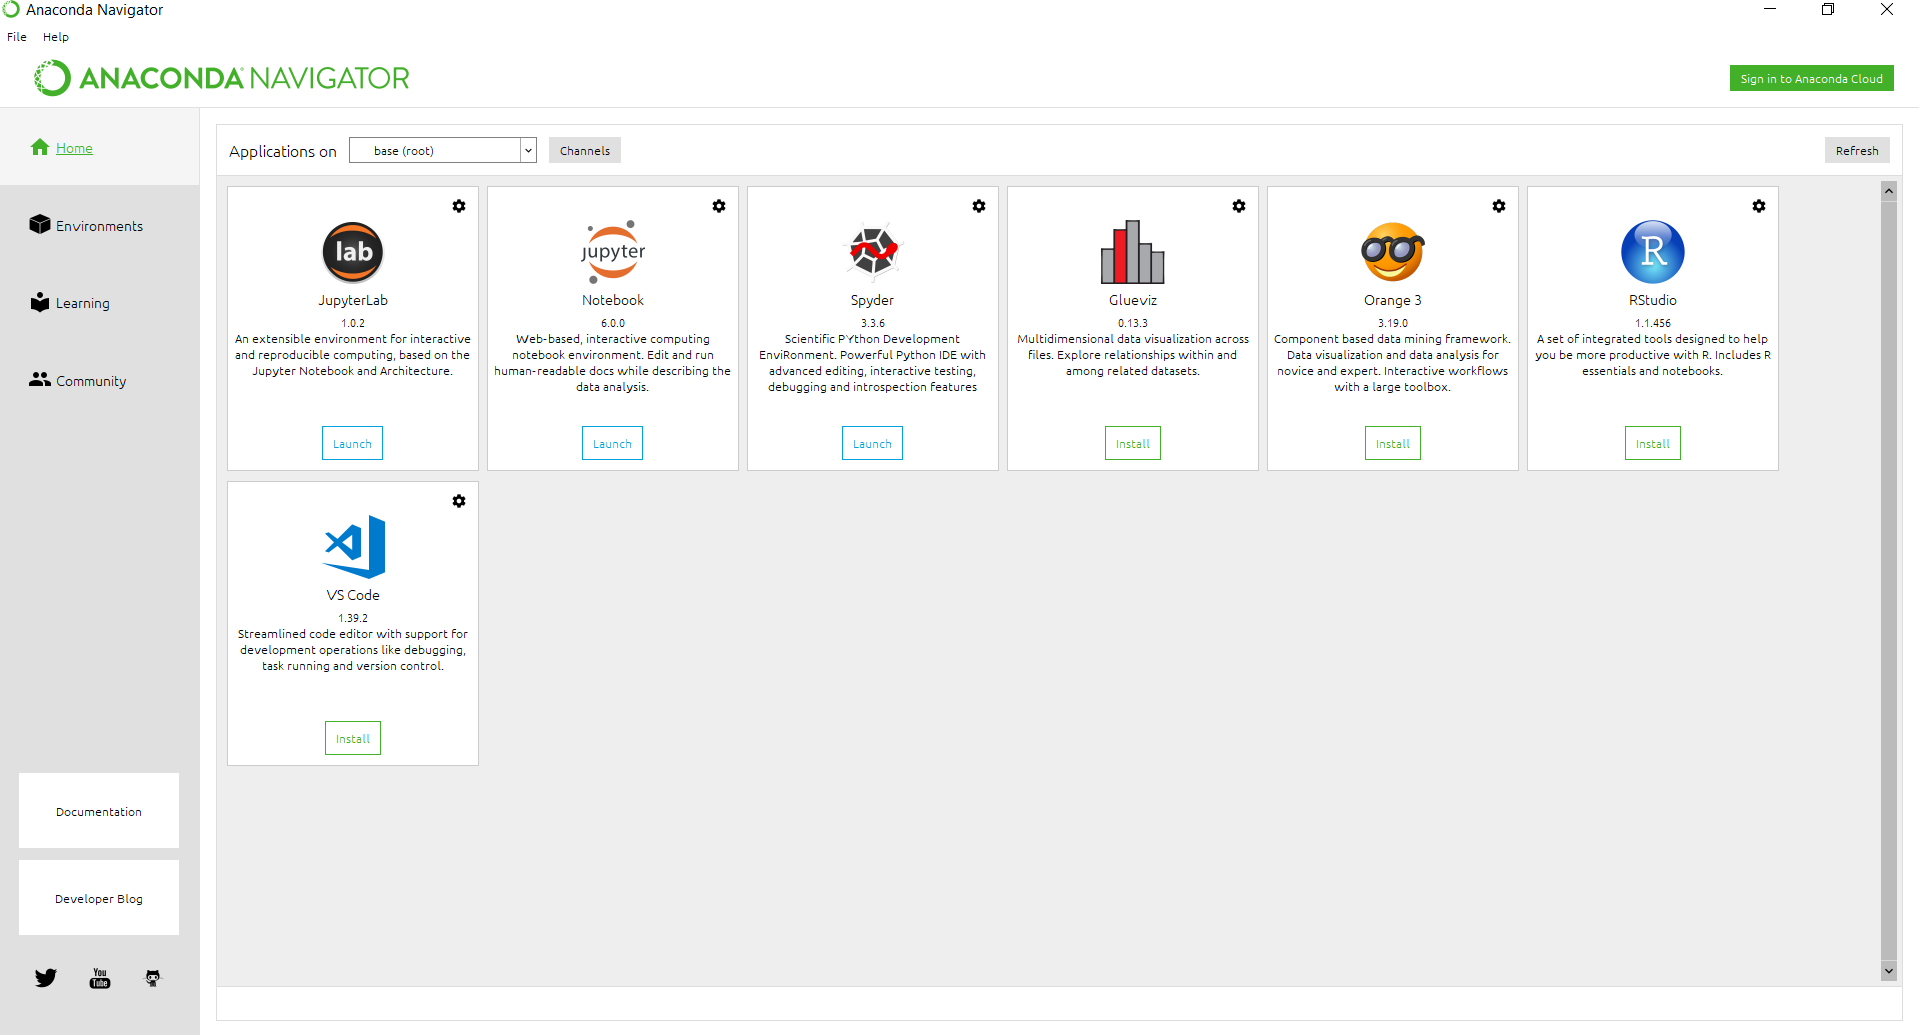
\includegraphics[scale=0.3]{figures/navigator}
    \caption{\textit{Launch Spider}}
    \label{Anaconda Navigator}
\end{figure}
\item ketikkan print("Hello World") dan run spyder dengan cara mengklik tombol berwarna hijau yang terletak ditengah toolbar, untuk lebih jelas dapat dilihat pada gambar \ref{Print Hello World}.
\begin{figure}[!htbp]
    \centering
    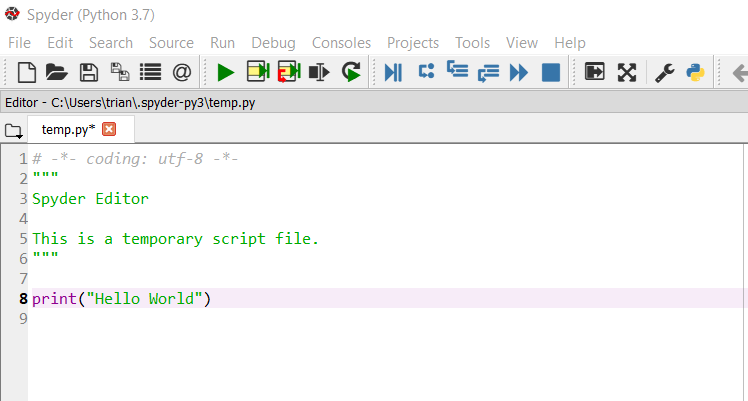
\includegraphics[scale=0.75]{figures/helloworld}
    \caption{\textit{Print Hello World}}
    \label{Print Hello World}
\end{figure}
\item hasilnya akan tampak seperti pada gambar \ref{Hello World}
\begin{figure}[!htbp]
    \centering
    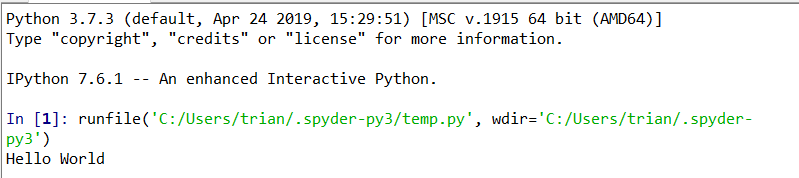
\includegraphics[scale=0.75]{figures/run}
    \caption{\textit{Hello World}}
    \label{Hello World}
\end{figure}
\end{enumerate}

\subsection{Pemakaian Variable Explorer}
Variable explorer akan secara otomatis terisi ketika kita membuat variable, pada variable explorer kita bisa melihat nama variable, tipe data, length, dan value dari variable tersebut. Contoh penggunaan variabel explorer dapat teman-teman lihat pada gambar \ref{Variable Explorer}.
\begin{figure}[!htbp]
    \centering
    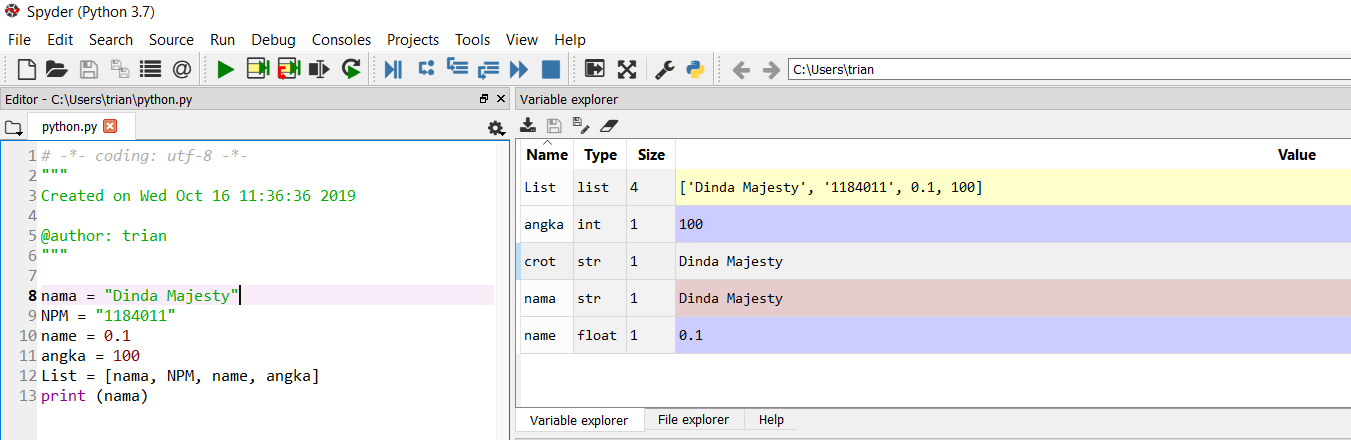
\includegraphics[scale=0.4]{figures/variable}
    \caption{\textit{Variable Explorer}}
    \label{Variable Explorer}
\end{figure}

\section{Indentasi}
\subsection{Penjelasan Indentasi}
Identasi adalah bagian paragraf yang menjorok ke dalam pada baris-baris paragraf. Mengatur indentasi dapat menggunakan tab atau spasi. Identasi digunakan oleh bahasa pemrograman python sebagai pengganti briket ({}) untuk membuka dan menutup fungsi. Error indentasi dapat terjadi apabila syntax tidak menggunakan tab atau space.
Contoh yang benar (menggunakan tab/spasi sebagai indentasi):
\begin{verbatim}
# blok percabangan if
if username == 'petanikode':
    print("Selamat Datang Admin")
    print("Silahkan ambil tempat duduk")

# blok percabangan for
for i in range(10):
    print i
\end{verbatim}
Contoh yang salah (tidak menggunakan tab/spasi):
\begin{verbatim}
# blok percabangan if
if username == 'petanikode':
print("Selamat Datang Admin")
print("Silahkan ambil tempat duduk")

# blok percabangan for
for i in range(10):
print i
\end{verbatim}

\subsection{Jenis-Jenis Error Indentasi}
IndentationError: unexpected indent. Error diatas terjadi apabila syntax kekurangan tab atau spasi. Contoh error identasi dapat dilihat pada gambar \ref{Indentasi}.
\begin{figure}[!htbp]
    \centering
    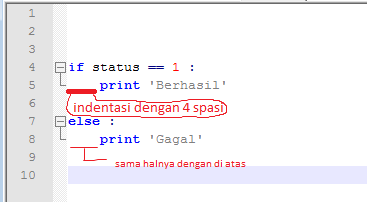
\includegraphics[scale=0.6]{figures/indentasi}
    \caption{\textit{Indentasi}}
    \label{Indentasi}
\end{figure}
Apabila di running akan memunculkan error seperti pada gambar \ref{Error Indentasi}.
\begin{figure}[!htbp]
    \centering
    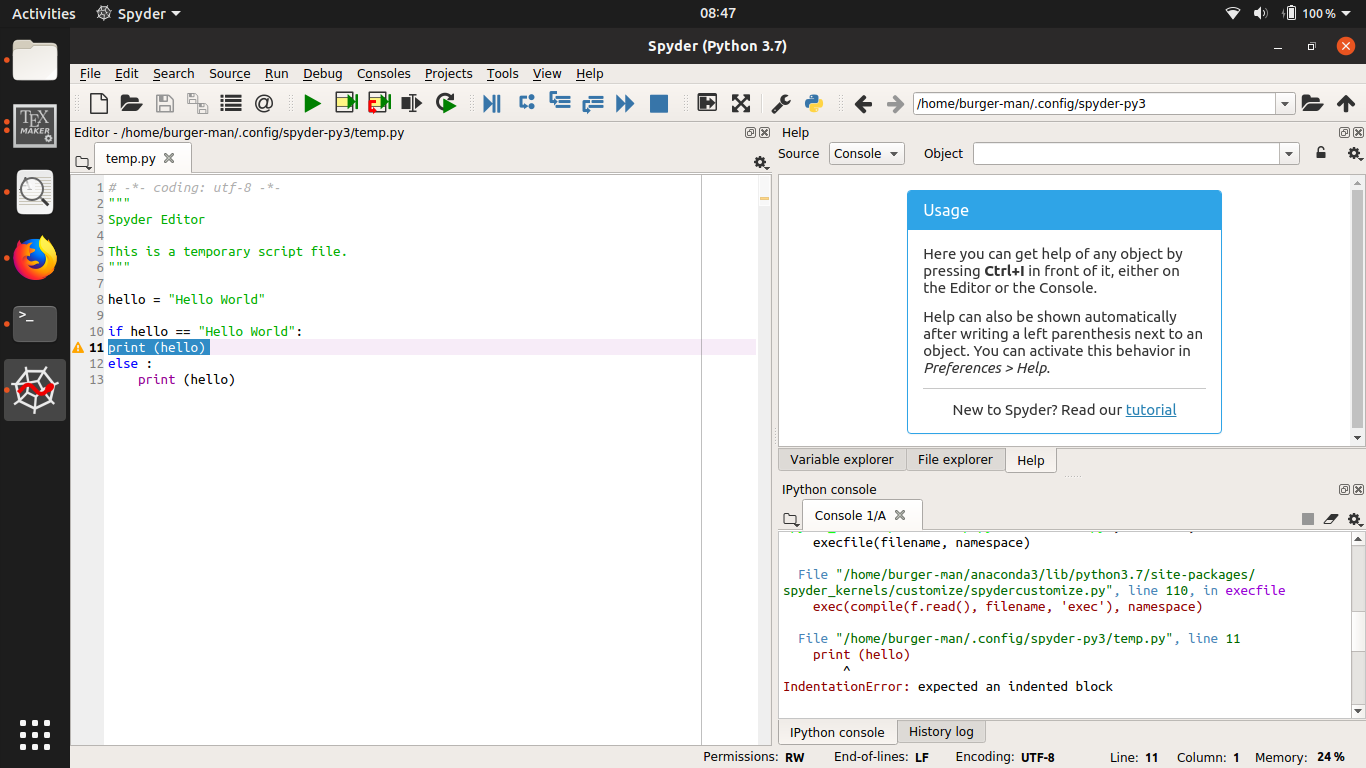
\includegraphics[scale=0.6]{figures/errorindentasi}
    \caption{\textit{Error Indentasi}}
    \label{Error Indentasi}
\end{figure}

\subsection{Cara Membaca Error}
Jika terjadi error maka cari di line berapa error terjadi, pada gambar \ref{Error Indentasi} terdapat error indentasi pada line 10.


\subsection{Cara Menangani Error}
Menangani error indentasi dapat dilakukan dengan cara menambahkan tab atau space pada line yang error. Untuk lebih jelasnya dapat teman-teman lihat pada gambar \ref{Syntax Error}.
\begin{figure}[H]
    \centering
    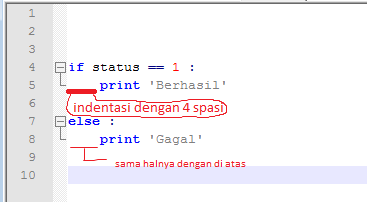
\includegraphics[scale=0.7]{figures/indentasi}
    \caption{\textit{Syntax Error}}
    \label{Syntax Error}
\end{figure}
Penulisan syntax identasi yang benar dapat dilihat pada gambar \ref{Syntax Error1}.
\begin{figure}[H]
    \centering
    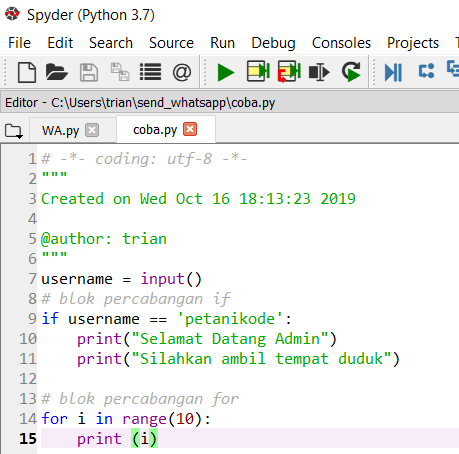
\includegraphics[scale=0.8]{figures/indentasicoy}
    \caption{\textit{Syntax yang Telah Diperbaiki}}
    \label{Syntax Error1}
\end{figure}

\subsection{Quiz: 1}
\begin{enumerate}
\item Siapakah pencipta Python?\\
a) Guido van Rossum\\
b) Guido van Persie\\
c) Guido van Linguini\\
d) Guido van Laptop

\item Pada tahun berapa python dikembangkan?\\
a) 1999\\
b) 1995\\
c) 1945\\
d) 1990

\item Apa itu indentasi?\\
a) Bagian paragraf yang menjorok ke dalam\\
b) Bagian paragraf yang menjorok ke sungai\\
c) Bagian paragraf yang menjorok ke laut\\
d) Bagian paragraf yang menjorok ke hati

\item Apa itu try except?\\
a) Perintah untuk penanganan masalah hidup\\
b) Perintah untuk penanganan masalah error\\
c) Perintah untuk penanganan masalah galau\\
d) Perintah untuk penanganan masalah sakit perut

\item Apa itu if statement?\\
a) Kondisi yang digunakan untuk percabangan logika\\
b) Kondisi yang digunakan untuk percabangan pohon\\
c) Kondisi yang digunakan untuk percabangan tunas\\
d) Kondisi yang digunakan untuk percabangan akar
\end{enumerate}